\chapter{Результаты работы программы}

\section{Методы фильтрации шумов}

Ниже представлены результаты фильтрации билатеральным методом при различных квадратных фильтрационных окнах.

\begin{figure}[h!]
	\centering
	\begin{minipage}{.5\textwidth}
		\centering
		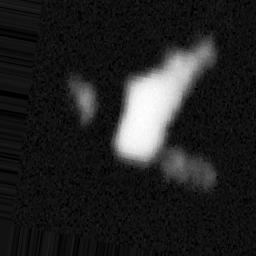
\includegraphics[width=0.8\linewidth]{inc/img/nc_original}
		\captionof{figure}{Исходное изображение}
		\label{fig:nc_original_0}
	\end{minipage}%
	\begin{minipage}{.5\textwidth}
		\centering
		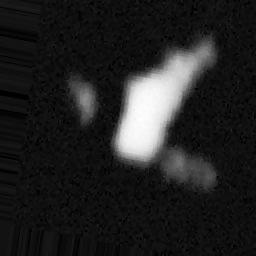
\includegraphics[width=0.8\linewidth]{inc/img/nc_b_s3}
		\captionof{figure}{3x3}
		\label{fig:nc_b_s3}
	\end{minipage}
\end{figure}

\begin{figure}[h!]
	\centering
	\begin{minipage}{.5\textwidth}
		\centering
		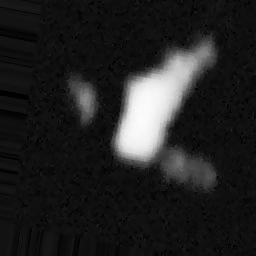
\includegraphics[width=0.8\linewidth]{inc/img/nc_b_s5}
		\captionof{figure}{5x5}
		\label{fig:nc_b_s5}
	\end{minipage}%
	\begin{minipage}{.5\textwidth}
		\centering
		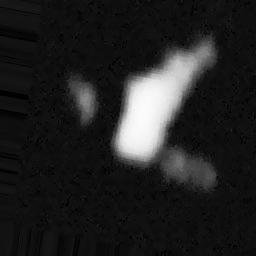
\includegraphics[width=0.8\linewidth]{inc/img/nc_b_s7}
		\captionof{figure}{7x7}
		\label{fig:nc_b_s7}
	\end{minipage}
\end{figure}

\newpage

Далее приведены примеры работы методов фильтрации при дисковом окне размера 10.

\begin{figure}[h!]
	\centering
	\begin{minipage}{.5\textwidth}
		\centering
		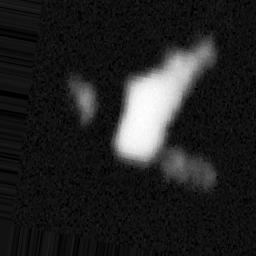
\includegraphics[width=0.8\linewidth]{inc/img/nc_original}
		\captionof{figure}{Исходное изображение}
		\label{fig:nc_original_1}
	\end{minipage}%
	\begin{minipage}{.5\textwidth}
		\centering
		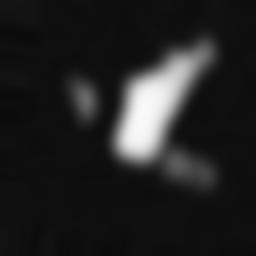
\includegraphics[width=0.8\linewidth]{inc/img/nc_mean_d10}
		\captionof{figure}{Фильтр среднего}
		\label{fig:nc_mean_d10}
	\end{minipage}
\end{figure}

\begin{figure}[h!]
	\centering
	\begin{minipage}{.5\textwidth}
		\centering
		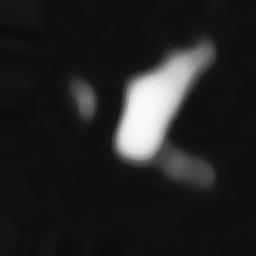
\includegraphics[width=0.8\linewidth]{inc/img/nc_m_d10}
		\captionof{figure}{Медианный фильтр}
		\label{fig:nc_m_d10}
	\end{minipage}%
	\begin{minipage}{.5\textwidth}
		\centering
		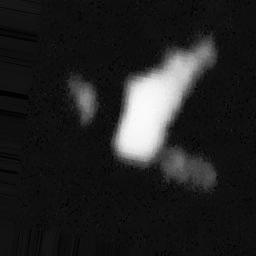
\includegraphics[width=0.8\linewidth]{inc/img/nc_b_d10}
		\captionof{figure}{Билатеральный фильтр}
		\label{fig:nc_b_d10}
	\end{minipage}
\end{figure}

\newpage

\section{Методы обратной свертки}

На рисунках \ref{fig:id_original}--\ref{fig:id_w} показаны результаты применения алгоритмов обратной свертки.

\begin{figure}[h!]
	\centering
	\begin{minipage}{.5\textwidth}
		\centering
		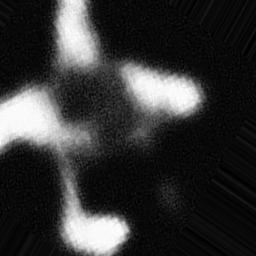
\includegraphics[width=0.8\linewidth]{inc/img/id_original}
		\captionof{figure}{Исходное изображение}
		\label{fig:id_original}
	\end{minipage}%
\end{figure}

\begin{figure}[h!]
	\centering
	\begin{minipage}{.5\textwidth}
		\centering
		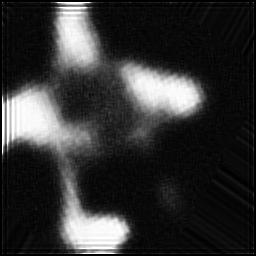
\includegraphics[width=0.8\linewidth]{inc/img/id_rl}
		\captionof{figure}{Ричардсон-Люси}
		\label{fig:id_rl}
	\end{minipage}%
	\begin{minipage}{.5\textwidth}
		\centering
		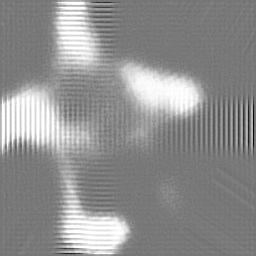
\includegraphics[width=0.8\linewidth]{inc/img/id_w}
		\captionof{figure}{Винер}
		\label{fig:id_w}
	\end{minipage}
\end{figure}

\newpage

\section{Методы повышения разрешения}

\begin{figure}[h!]
	\centering
	\begin{minipage}{.5\textwidth}
		\centering
		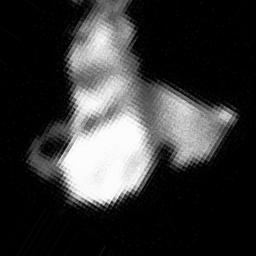
\includegraphics[width=0.2\linewidth]{inc/img/us_original}
		\captionof{figure}{Исходное изображение}
		\label{fig:us_original}
	\end{minipage}%
\end{figure}

\begin{figure}[h!]
	\centering
	\begin{minipage}{.5\textwidth}
		\centering
		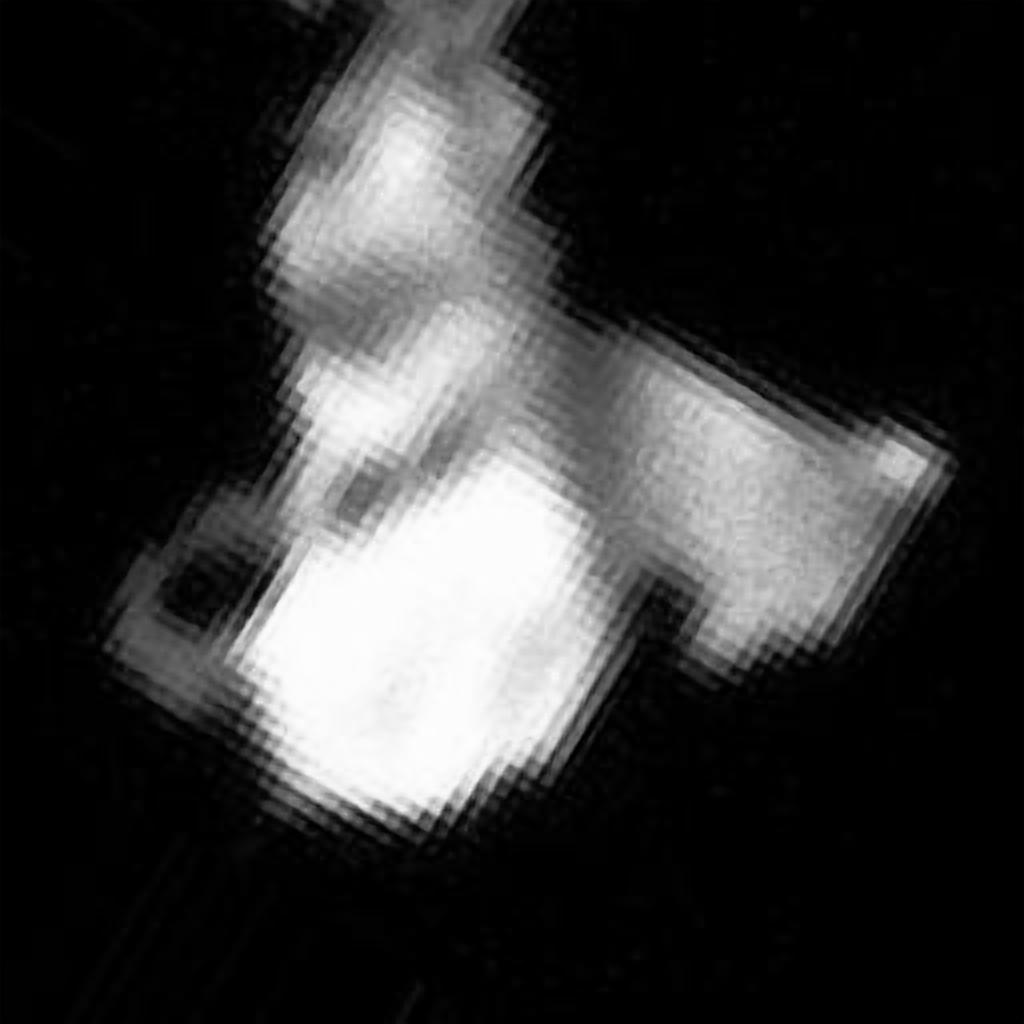
\includegraphics[width=0.8\linewidth]{inc/img/us_espcn_x4}
		\captionof{figure}{ESPCN x4}
		\label{fig:us_espcn_x4}
	\end{minipage}%
	\begin{minipage}{.5\textwidth}
		\centering
		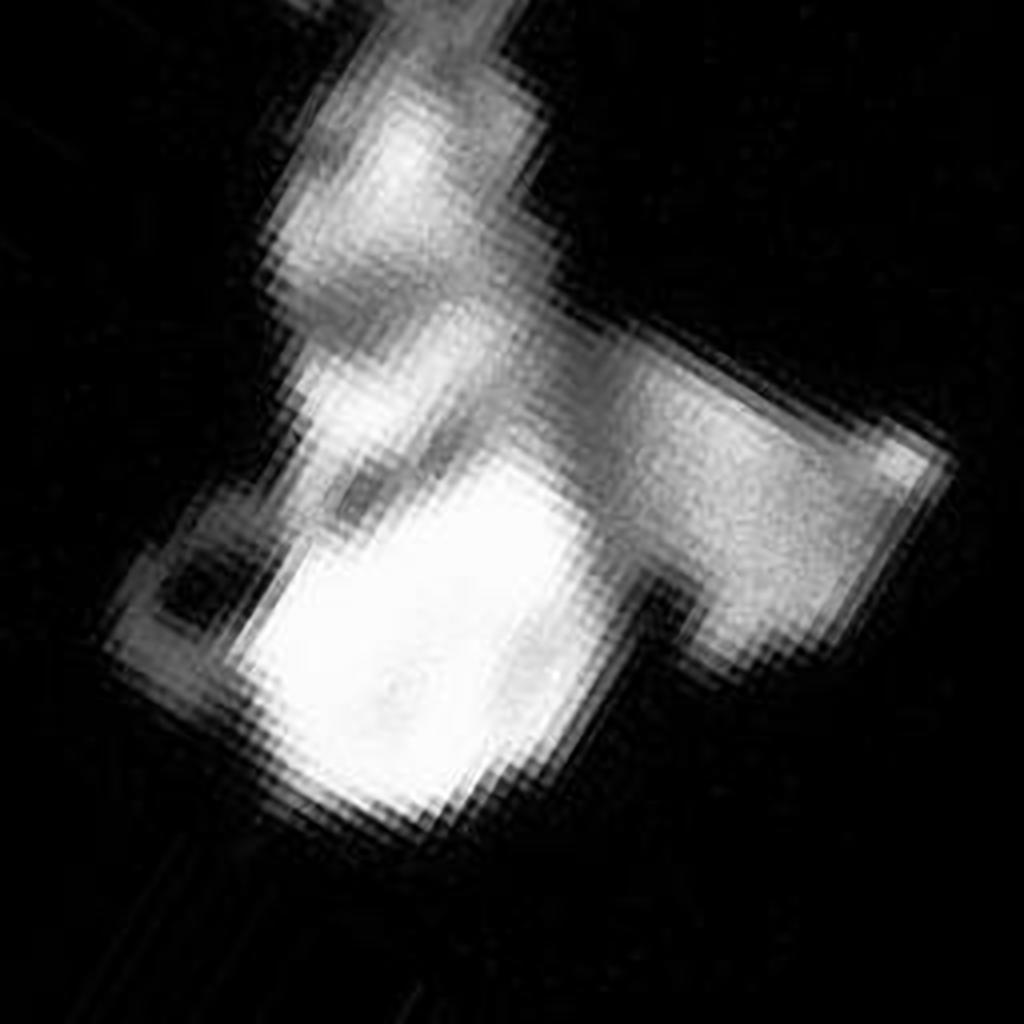
\includegraphics[width=0.8\linewidth]{inc/img/us_esdr_x4}
		\captionof{figure}{ESDR x4}
		\label{fig:us_esdr_x4}
	\end{minipage}
\end{figure}

\begin{figure}[h!]
	\centering
	\begin{minipage}{.5\textwidth}
		\centering
		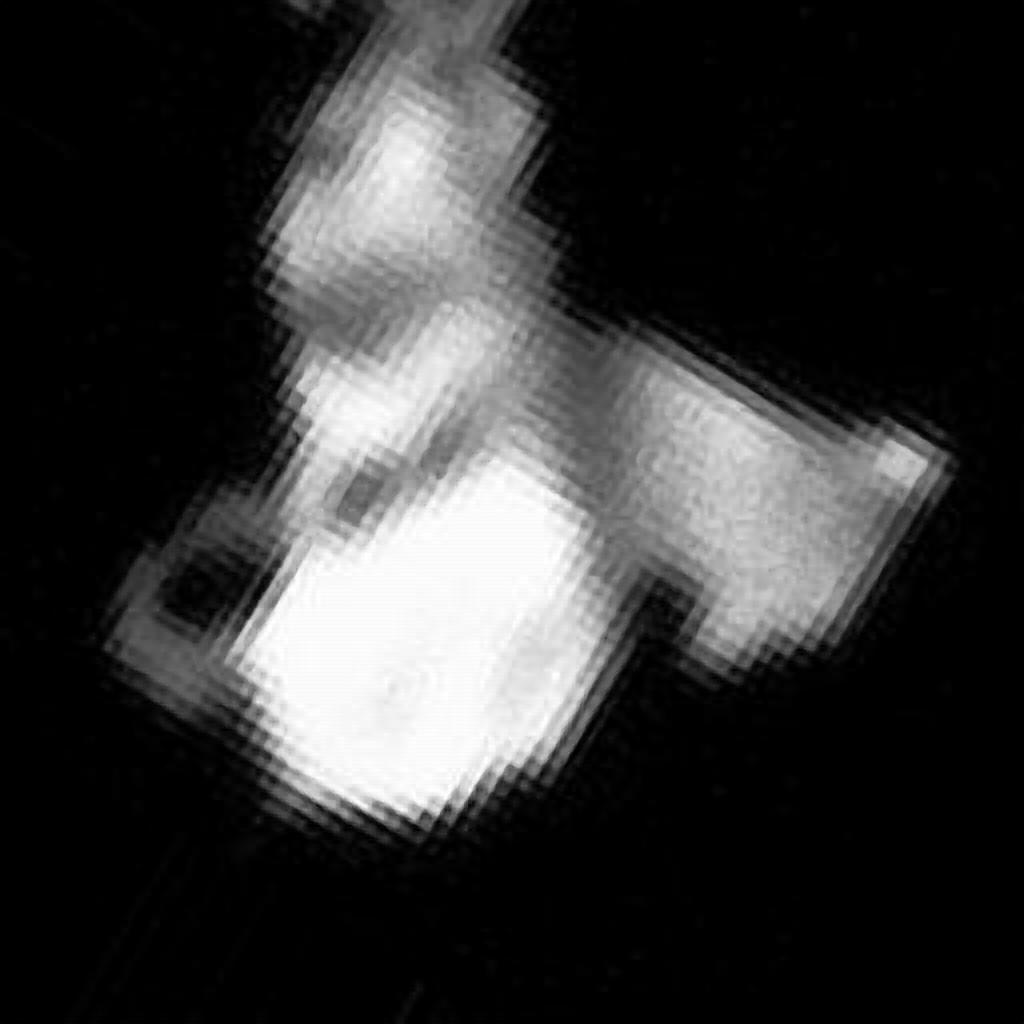
\includegraphics[width=0.8\linewidth]{inc/img/us_fsrcnn_x4}
		\captionof{figure}{FSRCNN x4}
		\label{fig:us_fsrcnn_x4}
	\end{minipage}%
	\begin{minipage}{.5\textwidth}
		\centering
		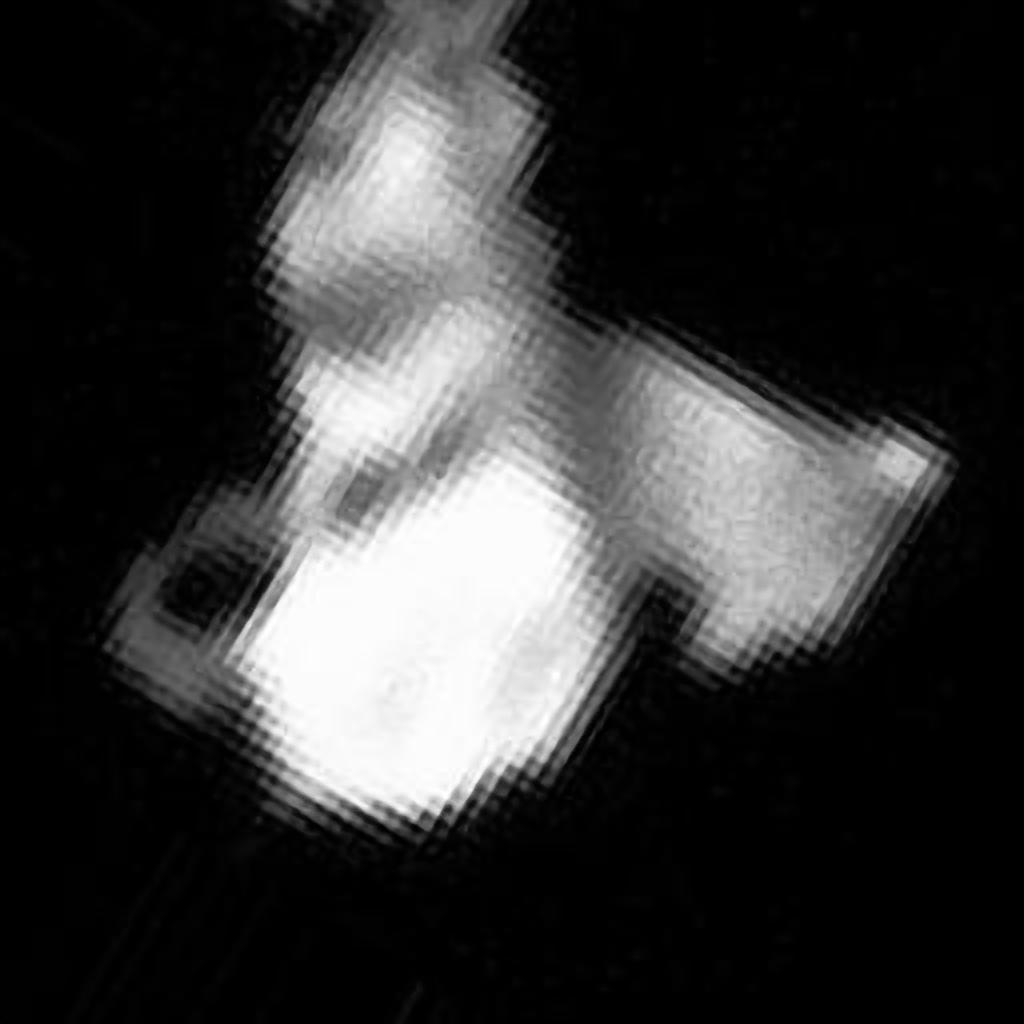
\includegraphics[width=0.8\linewidth]{inc/img/us_lapsrn_x4}
		\captionof{figure}{LapSRN x4}
		\label{fig:us_lapsrn_x4}
	\end{minipage}
\end{figure}

\section{Выводы}

Исходя из данных полученных в ходе тестирования можно сделать следующие выводы:
\begin{itemize}
	\item при фильтрации шумов на изображении следует учитывать характер шумов, в соответствии с которым должен производиться выбор размеров фильтрационного окна, т.к. в случае сильной зашумленности снимка фильтрационное окно необходимо увеличивать, иначе алгоритмы работают неэффективно;
	\item метод билатеральной фильтрации является наиболее предпочтительным поскольку позволяет сохранить четкие грани и больше деталей объектов на снимке даже в случае большого фильтрационного окна;
	\item алгоритмы обратной свертки требуют дальнейшей доработки путем добавления статистического анализа изображений для определения более близкой оценки функции рассеяния точки;
	\item на предложенных данных рассмотренные модели нейронных сетей для повышения разрешения показывают сопоставимые результаты ввиду низкой детализации исходных изображений, поэтому следует использовать быструю FSRCNN модель. Однако в случае дальнейшего развития аппаратной части наблюдений и повышения качества получаемых снимков стоит отдавать предпочтение LapSRN или EDSR моделям.
\end{itemize}
